\section{Communication technologies in Automotive Domain}
More than 100 ECUs connect via in-vehicle buses in modern vehicles\cite{b1.0}. As a result, there is a greater need than ever for a dependable communication network with high bandwidth. In order to meet these requirements, BMW implemented Ethernet for the first time in vehicles in 2013. At the same time, it is important to note that the incorporation of Ethernet as an in-vehicle networking system does not imply that traditional communication networks such as CAN, LIN, and MOST are rendered obsolete. Because these networks are robust, inexpensive, time-tested, and provide necessary performance for many applications, Automotive Ethernet will not completely replace them, but will supplement them to provide even more cost, performance, and feature benefits. Table \ref{tab:Comparison_Automotive_Networks} shows the important characteristics of automotive networks in comparison with the Ethernet.
\begin{center}
\begin{tabular}{|c|c|c|c|c|c|c}
\hline
\textbf{Property} & \textbf{Ethernet} & \textbf{CAN} & \textbf{FlexRay} & \textbf{MOST} & \textbf{LIN}\\
\hline
Bandwidth(Mb/s) & \textgreater 100 & 1 & 20 & 150 & 0.02\\
\hline
Nodes & Scalable & 30 & 22 & 64 & 16\\
\hline
Network Length & 15m per link & 40m & 24m & 1280m & 40m\\
\hline
%Media Access Control & Full-duplex contention less & Non-destructive arbitration & Time-triggered & Time-triggered & Time-triggered\\
Topologies & Star, Tree & Bus& Bus,start & Ring,Star & Bus\\
\hline
Cost & High& Low& Low& High& Very low\\
\hline
Cabling & UTP & UTP & UTP & Optical,UTP & 1-wire\\

\hline
\end{tabular}
\captionof{table}{Comparison of important characteristics of automotive networks \cite[p.202]{b1}}
\label{tab:Comparison_Automotive_Networks}
\end{center}

\section{Ethernet in the Automotive Domain}
\label{sec:EthernetInTheAutomotiveDomain}
In the year 1980, consumer-oriented Ethernet was introduced. However, Ethernet use in the automotive domain did not begin until 2013. This was due to EMC emissions levels being higher than those required for vehicle use. The introduction of BroadR-Reach twisted pair cables meant that the stringent EMC performance regulations were met and that the cables could finally be used in the automotive domain. Initially, Ethernet 100BASE-TX was used for OBD and updating the ECUs' flash memories\cite{b1.0.1_AE_History}. It has also been used for applications relating to infotainment and camera systems over the years. With an increasing number of sensors in a vehicle, data acquisition and high-speed communication become essential. In the current scenario, Automotive Ethernet appears to be the most viable solution for meeting these requirements. Also, Automotive Ethernet is said to be the next-generation in-vehicle networking systems when connecting application domains, transporting different kinds of data (control data, streaming, etc.)\cite{b1.0.1_AE_History}.  

\section{Ethernet as backbone in vehicles}
Traditionally, CAN, LIN, FlexRay, and MOST are used as in-vehicle communication technologies\cite{b1.0_EthBackbone}. Although Ethernet is a relatively new to the automotive domain, it offers several desirable properties such as high bandwidth, interoperability, robustness, low cost and seamless integration with the TCP/IP stack\cite{b1.0_EthBackbone}. Because it is a peer-to-peer network with full duplex communication, each ECU can communicate with one another at 100 Mb/s bandwidth. However, in order to meet the delay requirements, complementary technologies such as AVB for in-vehicle communication are required.   

\begin{figure}[!htb]
	\centering
		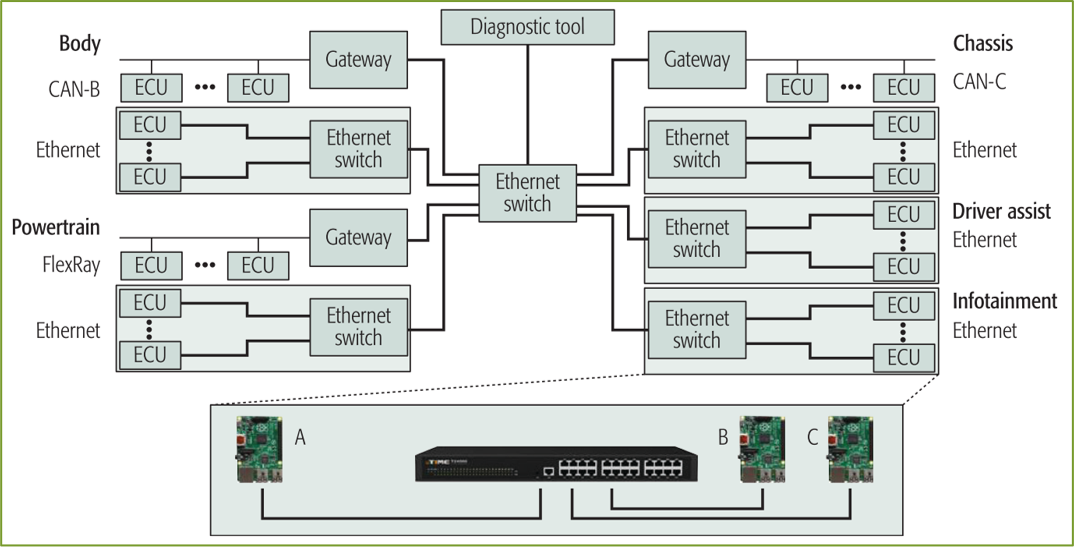
\includegraphics[width=1\textwidth]{images/Switched_Ethernet_backbone.png}
	\caption{Ethernet as a backbone for in-vehicle communication\cite{b1.0_EthBackbone}}
	\label{fig:Switched_Ethernet_backbone}
\end{figure}

\par Figure \ref{fig:Switched_Ethernet_backbone} is an example of an in-vehicle network with Ethernet as a backbone. Low-speed networks such as CAN, LIN, and Flexray are connected to Ethernet via a switch using gateways\cite{b1.0_EthBackbone}. This facilitates the establishment of a link between ECUs that are integrated with Ethernet as the native protocol and have higher bandwidth requirements for their applications, allowing message sharing across domains. With the introduction of IoT in the automotive industry, a switched Ethernet network serves as the foundation technology for implementing V2X communication.


\section{Service Oriented Architecture}
Automotive Ethernet has resulted in a paradigm shift in the development of automotive systems. Because scalability is one of the primary advantages of using Automotive Ethernet, newer protocols and technologies that provide smooth, flexible, and scalable software solutions are required. SOA is one of the tried-and-true web services technologies that can be applied in the automotive context to support the growing complexity of automotive software. Given the resource limitations of ECUs, the SOA protocols designed for high level machines and servers cannot be directly used for the automotive software. In order to bridge the gap and reuse the concepts of the existing SOA model, new protocols are needed to be developed. AUTOSAR provides a standardized specifications for a protocols such as SOME/IP and DDS which works by incorporating the concepts of the SOA model. The details of these technologies are discussed in the following section.   

\section{Middleware in the automotive domain}
The increasing complexity in the automotive applications means there is a need for standardized middleware that can provide common services and common interfaces to the application software components\cite{b_TrendsInACS}. Middleware is a software layer that connects and manages application components running on distributed hosts\cite{b_middleware}. In practice, a middleware is composed of a collection of existing communication protocols and carmarker-specific layers\cite{b_TrendsInACS}. In the context of communication control, the middleware's role is to provide a layer of abstraction between the application software and the network.\cite{b1.4}. AUTOSAR has standardized specifications for middleware such as SOME/IP and DDS. Apart from this several other middleware based on CAN protocol such as eSOC\cite{b_TrendsInACS} are available for use in the automotive context. 

\subsection{SOME/IP}
``Scalable service Oriented MiddlewarE over IP" abbreviated SOME/IP represents a middleware that was created for automotive use cases \cite{b1.1}. The compatibility with AUTOSAR was a necessity regarding SOME/IP at least on wire-format level \cite{b1.1}. SOME/IP communication is an exchange of messages between different devices like ECUs over IP \cite{b1.1}. The SOME/IP protocol aims to define a uniform middleware for IP-based communication within vehicles. Table \ref{ISO_OSI_Model} represents the organization of the SOME/IP middleware in the ISO/OSI model.
\par  

\begin{center}
		\begin{tabular}{|c|c|}
		\hline
			7 & \\
			6 & SOME/IP \\
			5 & \\
		\hline
			4 & TCP/UDP \\
		\hline
			3 & IPv4/IPv6 \\
		\hline
		2 & Eth.MAC/IEEE DLL \\
		\hline
		1 & Ethernet PHY \\
		\hline			
		\end{tabular}
	\captionof{table}{Simplified ISO/OSI model of Automotive Ethernet stack for communication control}
	\label{ISO_OSI_Model}
\end{center}

The protocol builds on top of an existing TCP/UDP stack, adding another level of abstraction for application communication by enabling locality transparency. This property denotes the fact that an application has no knowledge of which network node provides the desired function or information. If the desired function or information is available on the same ECU, a local connection is established between the software components \cite{b1.4}. When the information, on the other hand, is on another node on the same network, the middleware performs the necessary network communication and provides the data to the application.

\begin{figure}[!htb]
	\centering
		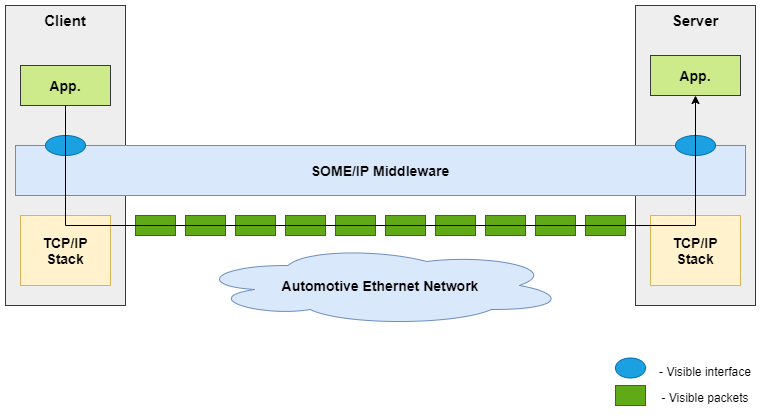
\includegraphics[width=1\textwidth]{images/SOMEIP_Middleware.png}
	\caption{SOA representation with SOME/IP middleware}
	\label{fig:SOMEIP_Middleware}
\end{figure}

Figure \ref{fig:SOMEIP_Middleware} depicts a high-level overview of the SOME/IP transformer. It is based on the client-server mechanism used in service-oriented architecture. This enables a variety of methods for sending and requesting data between the client and server via RPCs and Publish-Subscribe models. The following section describes the specifics of these communication methods.

\subsubsection{Communication methods}
\label{sec:CommunicationMethods}

\begin{figure}[!htb]
	%\centering
		\begin{subfigure}[b]{.5\textwidth}
		%	\centering
				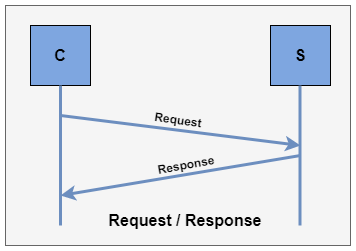
\includegraphics[width=\textwidth]{images/Request-response.png}
				\caption{``Request-Response"'-RPC: method call with response message}
				\label{fig:Request-response}
		\end{subfigure}		
		\begin{subfigure}[b]{.5\textwidth}
		%	\centering
			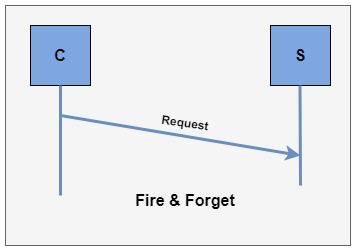
\includegraphics[width=\textwidth]{images/fire-forget.png}
			\caption{``Fire \& Forget"'- RPC: Method call without a response}
			\label{fig:fire-forget}
		\end{subfigure}
		\begin{subfigure}[b]{.5\textwidth}
			%\centering
				 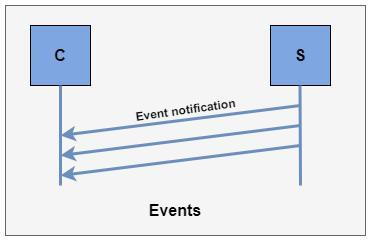
\includegraphics[width=\textwidth]{images/Events.png}
				\caption{``Publish-Subscribe - Events"': Event notifications}
				%\caption{fig 1}
				\label{fig:Events}
		\end{subfigure}
		\begin{subfigure}[b]{.5\textwidth}
			%\centering
				 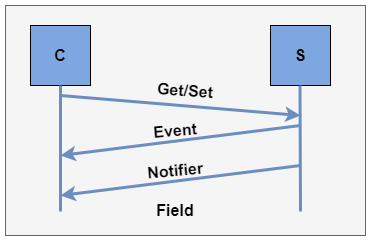
\includegraphics[width=\textwidth]{images/Field.png}
				\caption{``Fields"': Set or read out the data fields of
another service.}
				%\caption{fig 1}
				\label{fig:Field}
		\end{subfigure}
	\caption{SOME/IP communication types between clients and servers}
\end{figure}








